\section{Brief Description of Hardware Components in Arduino Portenta H7}

Here's a comprehensive list of hardware parts commonly found in the Arduino Portenta H7 see Figure ~\ref{PortentaH7Hardware}.

\begin{figure}
		\begin{center}
		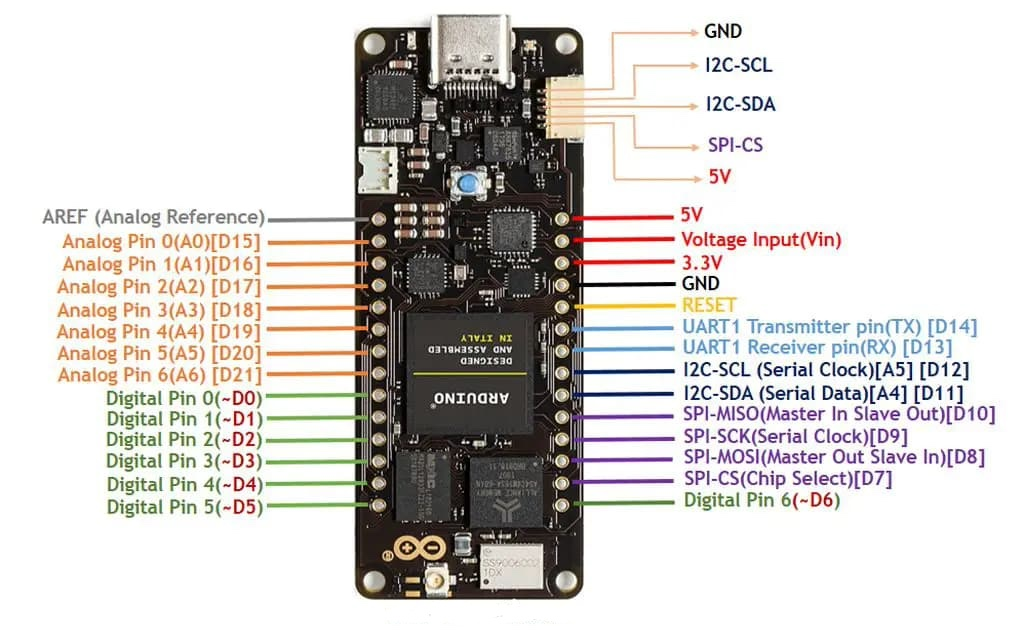
\includegraphics[width=0.7\linewidth]{images/ArduinoIDE/ArduinoHardware.jpg}
		\captionof{figure}{PortentaH7 Hardware}
		\label{PortentaH7Hardware}
		\cite{portentaH7doc:2024}
	\end{center}
\end{figure}

\begin{enumerate}
	\item \textbf{Microcontroller Unit (MCU):} The MCU is the main processing unit of the Arduino Portenta H7. It consists of a powerful dual-core STM32H747 processor, with an Arm Cortex-M7 core running at up to 480 MHz and an Arm Cortex-M4 core running at up to 240 MHz. This dual-core architecture provides the device with significant processing power and flexibility for handling complex tasks and applications. \cite{arduinoABX00042:2024} 
	
	\item \textbf{Memory:} The Arduino Portenta H7 supports various types of memory to accommodate different requirements for program storage and data manipulation. Here are the main varieties of memory available in the Portenta H7:
	
	\begin{itemize}
		\item \textbf{Flash Memory:} Ideal for storing program code and non-volatile data, ensuring data retention even during power loss.
		
		\item \textbf{RAM (Random Access Memory):} Offers speedy access for runtime data and variable storage during program execution.
		
		\item \textbf{External Storage:} Supports expansion via external storage devices like SD cards, facilitating additional space for large datasets and multimedia content.
		
		\item \textbf{Cache Memory:} Enhances performance by temporarily storing frequently accessed data and instructions close to the CPU cores, reducing memory access latency.
	\end{itemize}
	
	
	\item \textbf{Connectivity Interfaces:} The Portenta H7 offers a variety of connectivity options, including Ethernet, Wi-Fi, Bluetooth, USB, and serial interfaces such as SPI, I2C, UART, and CAN bus. These interfaces enable the device to communicate with other devices, sensors, actuators, and networks, facilitating data exchange, control, and networking capabilities.
	
	\item \textbf{I/O Pins:} The Arduino Portenta H7 provides a variety of I/O (Input/Output) pins, both digital and analog, offering flexibility for interfacing with external components and peripherals \cite{arduinoABX00042:2024}. Here are the different types of I/O pins available in the Portenta H7:
	
	\begin{itemize}
		
		\item \textbf{Digital I/O Pins:} These pins (D0 to D6 green color in above figure ~\ref{PortentaH7Hardware}) can be configured as either input or output and are used for digital communication or controlling digital devices. They typically support binary states, either HIGH (5V) or LOW (0V).
		
		\item \textbf{Analog Input Pins:} The Portenta H7 features analog input pins (A0 to A6 orange color in above figure ~\ref{PortentaH7Hardware}) that can measure continuous voltage levels. These pins are often used to interface with analog sensors or read analog signals from external devices. They provide a range of values rather than discrete digital states.
		
		\item \textbf{PWM (Pulse Width Modulation) Pins:} Some of the digital I/O pins on the Portenta H7 support PWM output. PWM pins can generate analog-like signals with varying duty cycles, allowing for control of devices such as motors or LED brightness.
		
		\item \textbf{I2C (Inter-Integrated Circuit) Pins:} I2C pins ( dark-blue color pins in ~\ref{PortentaH7Hardware}) allow for serial communication with devices using the I2C protocol. This communication protocol enables multiple devices to communicate with each other using only two wires, making it suitable for connecting sensors, displays, and other peripherals.
		
		\item \textbf{SPI (Serial Peripheral Interface) Pins:} SPI pins (purple color pins in ~\ref{PortentaH7Hardware}) facilitate high-speed serial communication between the Portenta H7 and other devices using the SPI protocol. SPI is commonly used to interface with devices such as SD cards, displays, and sensors that require fast data transfer rates.
		
		\item \textbf{UART (Universal Asynchronous Receiver-Transmitter) Pins:} UART pins (blue color pins in ~\ref{PortentaH7Hardware}) provide serial communication capabilities for transmitting and receiving data asynchronously between the Portenta H7 and other devices. UART is widely used for communication between microcontrollers, sensors, GPS modules, and other peripherals.
		
		\item \textbf{CAN (Controller Area Network) Pins:} The Portenta H7 may include CAN pins for communication over the Controller Area Network protocol. CAN is commonly used in automotive and industrial applications for robust, high-speed communication between devices in a network.
		
	\end{itemize}
	
	
	
	\item \textbf{Analog-to-Digital Converter (ADC):} The ADC allows the Portenta H7 to convert analog signals from sensors or other external devices into digital values that can be processed by the system. This enables the device to interface with analog sensors and acquire analog data for processing and analysis. Here are some common types of ADCs that may be available in the Portenta H7 \cite{arduinoABX00042:2024} :
	
	\begin{itemize}
		
		\item \textbf{Single-Channel ADCs:} These ADCs have a single input channel, making them suitable for applications that only require the conversion of a single analog signal.
		
		\item \textbf{Multi-Channel ADCs:} These ADCs have multiple input channels, allowing them to simultaneously convert multiple analog signals. This is useful for applications that involve monitoring multiple sensors or acquiring data from multiple sources.
		
		\item \textbf{Differential ADCs:} These ADCs measure the voltage difference between two input channels, providing higher accuracy and noise immunity compared to single-ended ADCs. They are suitable for applications that require precise measurements or operate in noisy environments.
		
		\item \textbf{High-Resolution ADCs:} These ADCs offer higher resolution, typically with more bits of resolution, allowing them to capture finer details in the analog signal. This is beneficial for applications that require high accuracy or deal with low-level signals.
		
		\item \textbf{High-Speed ADCs:} These ADCs can sample analog signals at high speeds, enabling them to capture rapidly changing signals or high-frequency signals. They are suitable for applications that require real-time data acquisition or signal processing.
		
		\item \textbf{Low-Power ADCs:} These ADCs consume minimal power during operation, making them suitable for battery-powered or energy-efficient applications. They optimize power consumption while maintaining adequate performance.
		
		\item \textbf{Integrated ADCs with Signal Conditioning:} Some variants of the Portenta H7 may include integrated ADCs with built-in signal conditioning features such as programmable gain amplifiers (PGAs), filters, or input multiplexers. These features enhance the ADC's functionality and performance, simplifying the design of analog front-end circuits.	
		
	\end{itemize}
	
	
	
	\item \textbf{Digital-to-Analog Converter (DAC):} The DAC enables the Portenta H7 to convert digital signals into analog voltages or currents, facilitating control over analog devices like motors, actuators, or audio amplifiers. While the Portenta H7 doesn't have built-in DACs, external DAC modules or shields can be added for this functionality. Examples include modules like MCP4922, ADS1115, DAC8831, and DAC7564, which offer varying resolutions and channels for interfacing with the Portenta H7 \cite{arduinoABX00042:2024}.
	
	\item \textbf{Real-Time Clock (RTC):} The RTC is a dedicated hardware component that keeps track of the current date and time, even when the device is powered off. This enables the Portenta H7 to perform timekeeping functions, schedule tasks, and timestamp data with accurate time information \cite{arduinoABX00042:2024}.
	
	\item \textbf{Secure Element/TrustZone:} Some variants of the Portenta H7 may include hardware-based security features such as a secure element or TrustZone technology. These security features provide hardware-based protection for sensitive data, cryptographic operations, and secure boot processes, enhancing the device's security against unauthorized access and attacks.
	
	\item \textbf{Power Management Unit (PMU):} The PMU is responsible for managing the power distribution and consumption within the device. It typically includes voltage regulators, power switches, and monitoring circuits to ensure efficient power usage, regulate voltage levels, and protect the system from power-related issues such as overvoltage, undervoltage, or overcurrent conditions \cite{arduinoABX00042:2024}.
	
	\item \textbf{Peripherals and Expansion Interfaces:} The Portenta H7 may feature various peripherals and expansion interfaces to support additional functionality and connectivity options. These peripherals may include SD card slots, audio codecs, cryptographic accelerators, motor control interfaces, and more. Additionally, the device may offer expansion interfaces such as GPIO headers, expansion slots, or mezzanine connectors for attaching external modules, shields, or custom expansion boards to extend its capabilities.
\end{enumerate}

\begin{comment}
	
	\section{Hardware Installation}
	
	To begin using the Arduino Portenta H7, follow these steps:
	
	\textbf{Hardware and Software Requirements:}
	
	\begin{itemize}
		\item Arduino Portenta H7 board
		\item USB type- C cable
		\item Arduino IDE 2.3.2 or newer version
	\end{itemize}
	
	\textbf{Procedure:}
	
	\begin{enumerate}
		\item Connect the Arduino Portenta H7 board to your laptop using a USB Type-C cable. When connected, the LED on the board should start blinking green, indicating that it is powered and connected to the laptop.
		
		\item If the board does not respond via USB, double-press the reset button. This action will reset the board and put it into bootloader mode. The LED should start blinking again, indicating that the board is ready for use.
		
		\item Ensure that you have the Arduino IDE installed on your laptop. Version 2.3.2 or a newer version is recommended.
		
		\item If you plan to use the Arduino Vision Shield, connect it to the Arduino Portenta H7 using the high-density connectors provided. The Vision Shield is designed to sit on top of the Arduino Portenta boards, expanding their capabilities for machine vision applications.
		
		\item Once the hardware connections are established, you can start programming the Arduino Portenta H7 using the Arduino IDE. Write your code, upload it to the board, and test your projects.
	\end{enumerate}
	
\end{comment}


%	The PortentaH7 is a high-performance microcontroller board developed by Arduino. It is designed to cater to professional applications, offering robust computing power, advanced features, and versatility. Here are some key aspects of the PortentaH7:

%	Within the H7 family, there are two variants; H7 Lite and H7 Lite Connected. All the three boards and their differences are presented in this datasheet.

%	\textbf{Target Areas}: 
%	Laboratory equipment, Computer vision

%	\begin{figure}
	%	\begin{center}
		%			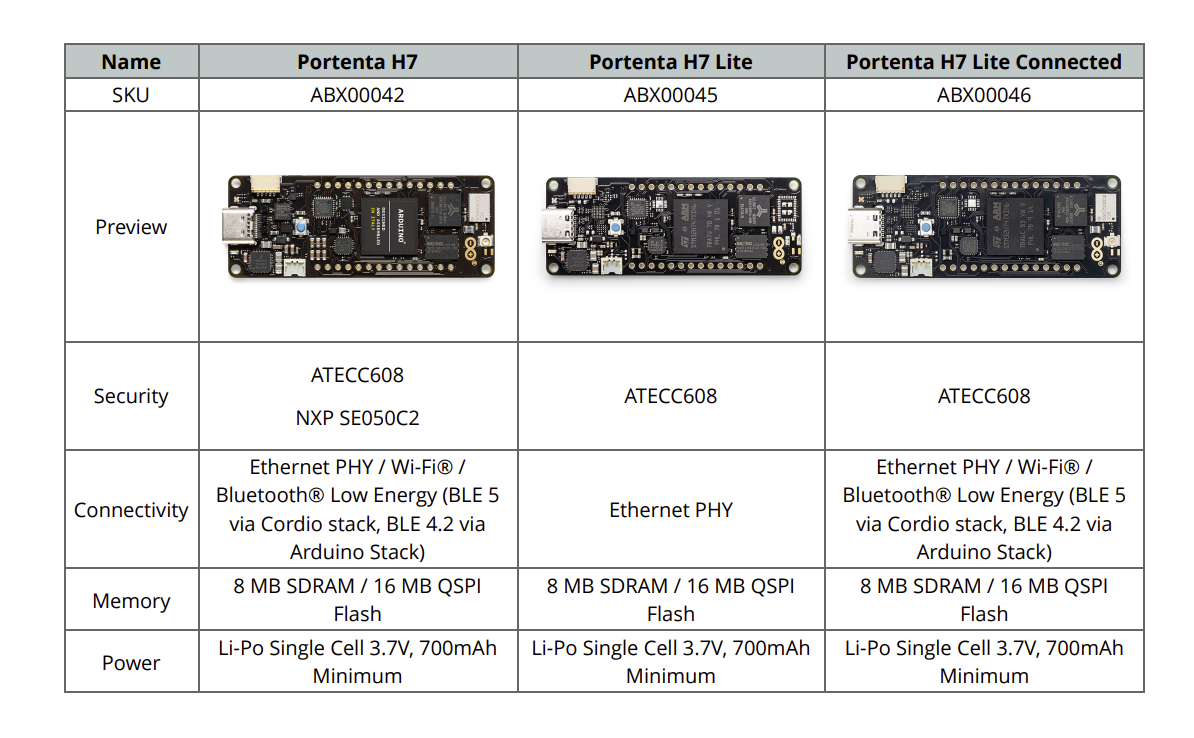
\includegraphics[width=0.7\linewidth]{Images/PortentaH7/TypesofPortentaH7.png}
		%			\caption{Types of PortentaH7}
		%			\label{Types}
		%	\end{center}
	%	\end{figure}

%\section{Key Features:}

%\textbf{Dual-core Processor:}

%\begin{itemize}
%	\item Cortex-M7: Runs at up to 480 MHz.
%	\item Cortex-M4: Runs at up to 240 MHz.
%	\item These cores can operate simultaneously, allowing for efficient parallel processing and real-time application execution.
%\end{itemize}

%\textbf{Memory:}
%\begin{itemize}
%\item RAM: 1 MB of SRAM and 16 MB of SDRAM.
%\item Flash Storage: 8 MB.
%\end{itemize}

%\textbf{Connectivity:}
%\begin{itemize}
%\item $<$ Built-in GPU for handling advanced graphical interfaces. 
%\item $<$ Supports an external display through a dedicated connector.
%\end{itemize}

%\textbf{Security:}
%\begin{itemize}
%\item Hardware cryptography support for secure applications.
%\item Secure boot and secure firmware updates.
%\end{itemize}

%\textbf{Expansion Options:}
%\begin{itemize}
%\item Compatible with Arduino MKR and \textbf{Portenta Vision Shield.}
%\item High-density connectors for custom hardware extensions.
%\end{itemize}

%\textbf{Operating Systems:}
%\begin{itemize}
%\item Capable of running high-level OS like Arm Mbed OS or real-time operating systems (RTOS).
%\item Compatible with Arduino programming environment and libraries.
%\end{itemize}

%\textbf{Power Management:}
%\begin{itemize}
%\item Multiple power supply options: USB-C, Li-Po battery, or external sources.
%\item Low power modes for energy-efficient applications.
%\end{itemize}

%\textbf{Applications:} \newline
%	The Portenta H7 is suitable for a wide range of professional applications, including but not limited to:

%\begin{itemize}
%	\item \textbf{Industrial IoT:} Real-time monitoring, data acquisition, and control systems.
%	\item \textbf{Edge Computing:} Local data processing and decision-making.
%	\item \textbf{AI and Machine Learning:} On-device inference and analytics.
%	\item \textbf{Robotics:} Advanced motor control and sensor integration.
%	\item \textbf{Smart Devices:} Connected appliances, home automation, and wearables.
%\end{itemize}

\begin{comment}

\section{Configuration of Arduino IDE}

In this section we will be looking at how to connect the Arduino Portenta H7 with a PC/laptop in order to use the board. Then, we will be going through the first steps of installing the relevant packages to use the Arduino Portenta H7 board and then we will be implementing a basic example sketch from the Arduino IDE.

\subsection{Step-wise Configuration}

\begin{enumerate}
	
	\item Connect the Arduino Portenta H7 board to the computer via USB Type-C cable.
	
	\item Press the reset button twice on the board and the LED on the board starts blinking green as shown in the Figure \ref{Arduino PortentaH7 Connected to a Laptop} indicating that it is ready.
	
	\begin{figure}
		\begin{center}
			
			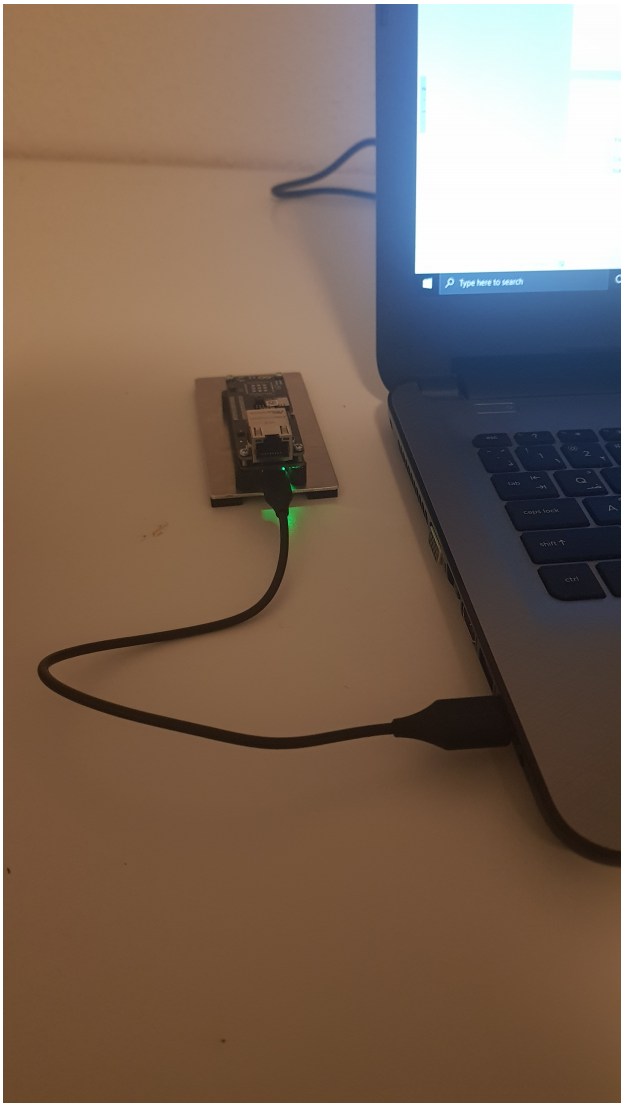
\includegraphics[width=0.4\linewidth]{images/ArduinoIDE/ArduinoPortentaH7Connectedtoalaptop.png}
			\captionof{figure}{Arduino PortentaH7 Connected to a Laptop}
			\label{Arduino PortentaH7 Connected to a Laptop}
		\end{center}
		
	\end{figure}
	
	\item Next, open the Arduino IDE and navigate to the Boards Manager by selecting \SHELL{Tools > Board > Boards Manager}. In the Boards Manager, search for "Portenta," select \textbf{Arduino Mbed OS Portenta Boards}, and click "Install". Fig \ref{Installation Arduino Mbed OS Portenta Board} 
\end{enumerate}	

\begin{figure}
	\begin{center}
		
		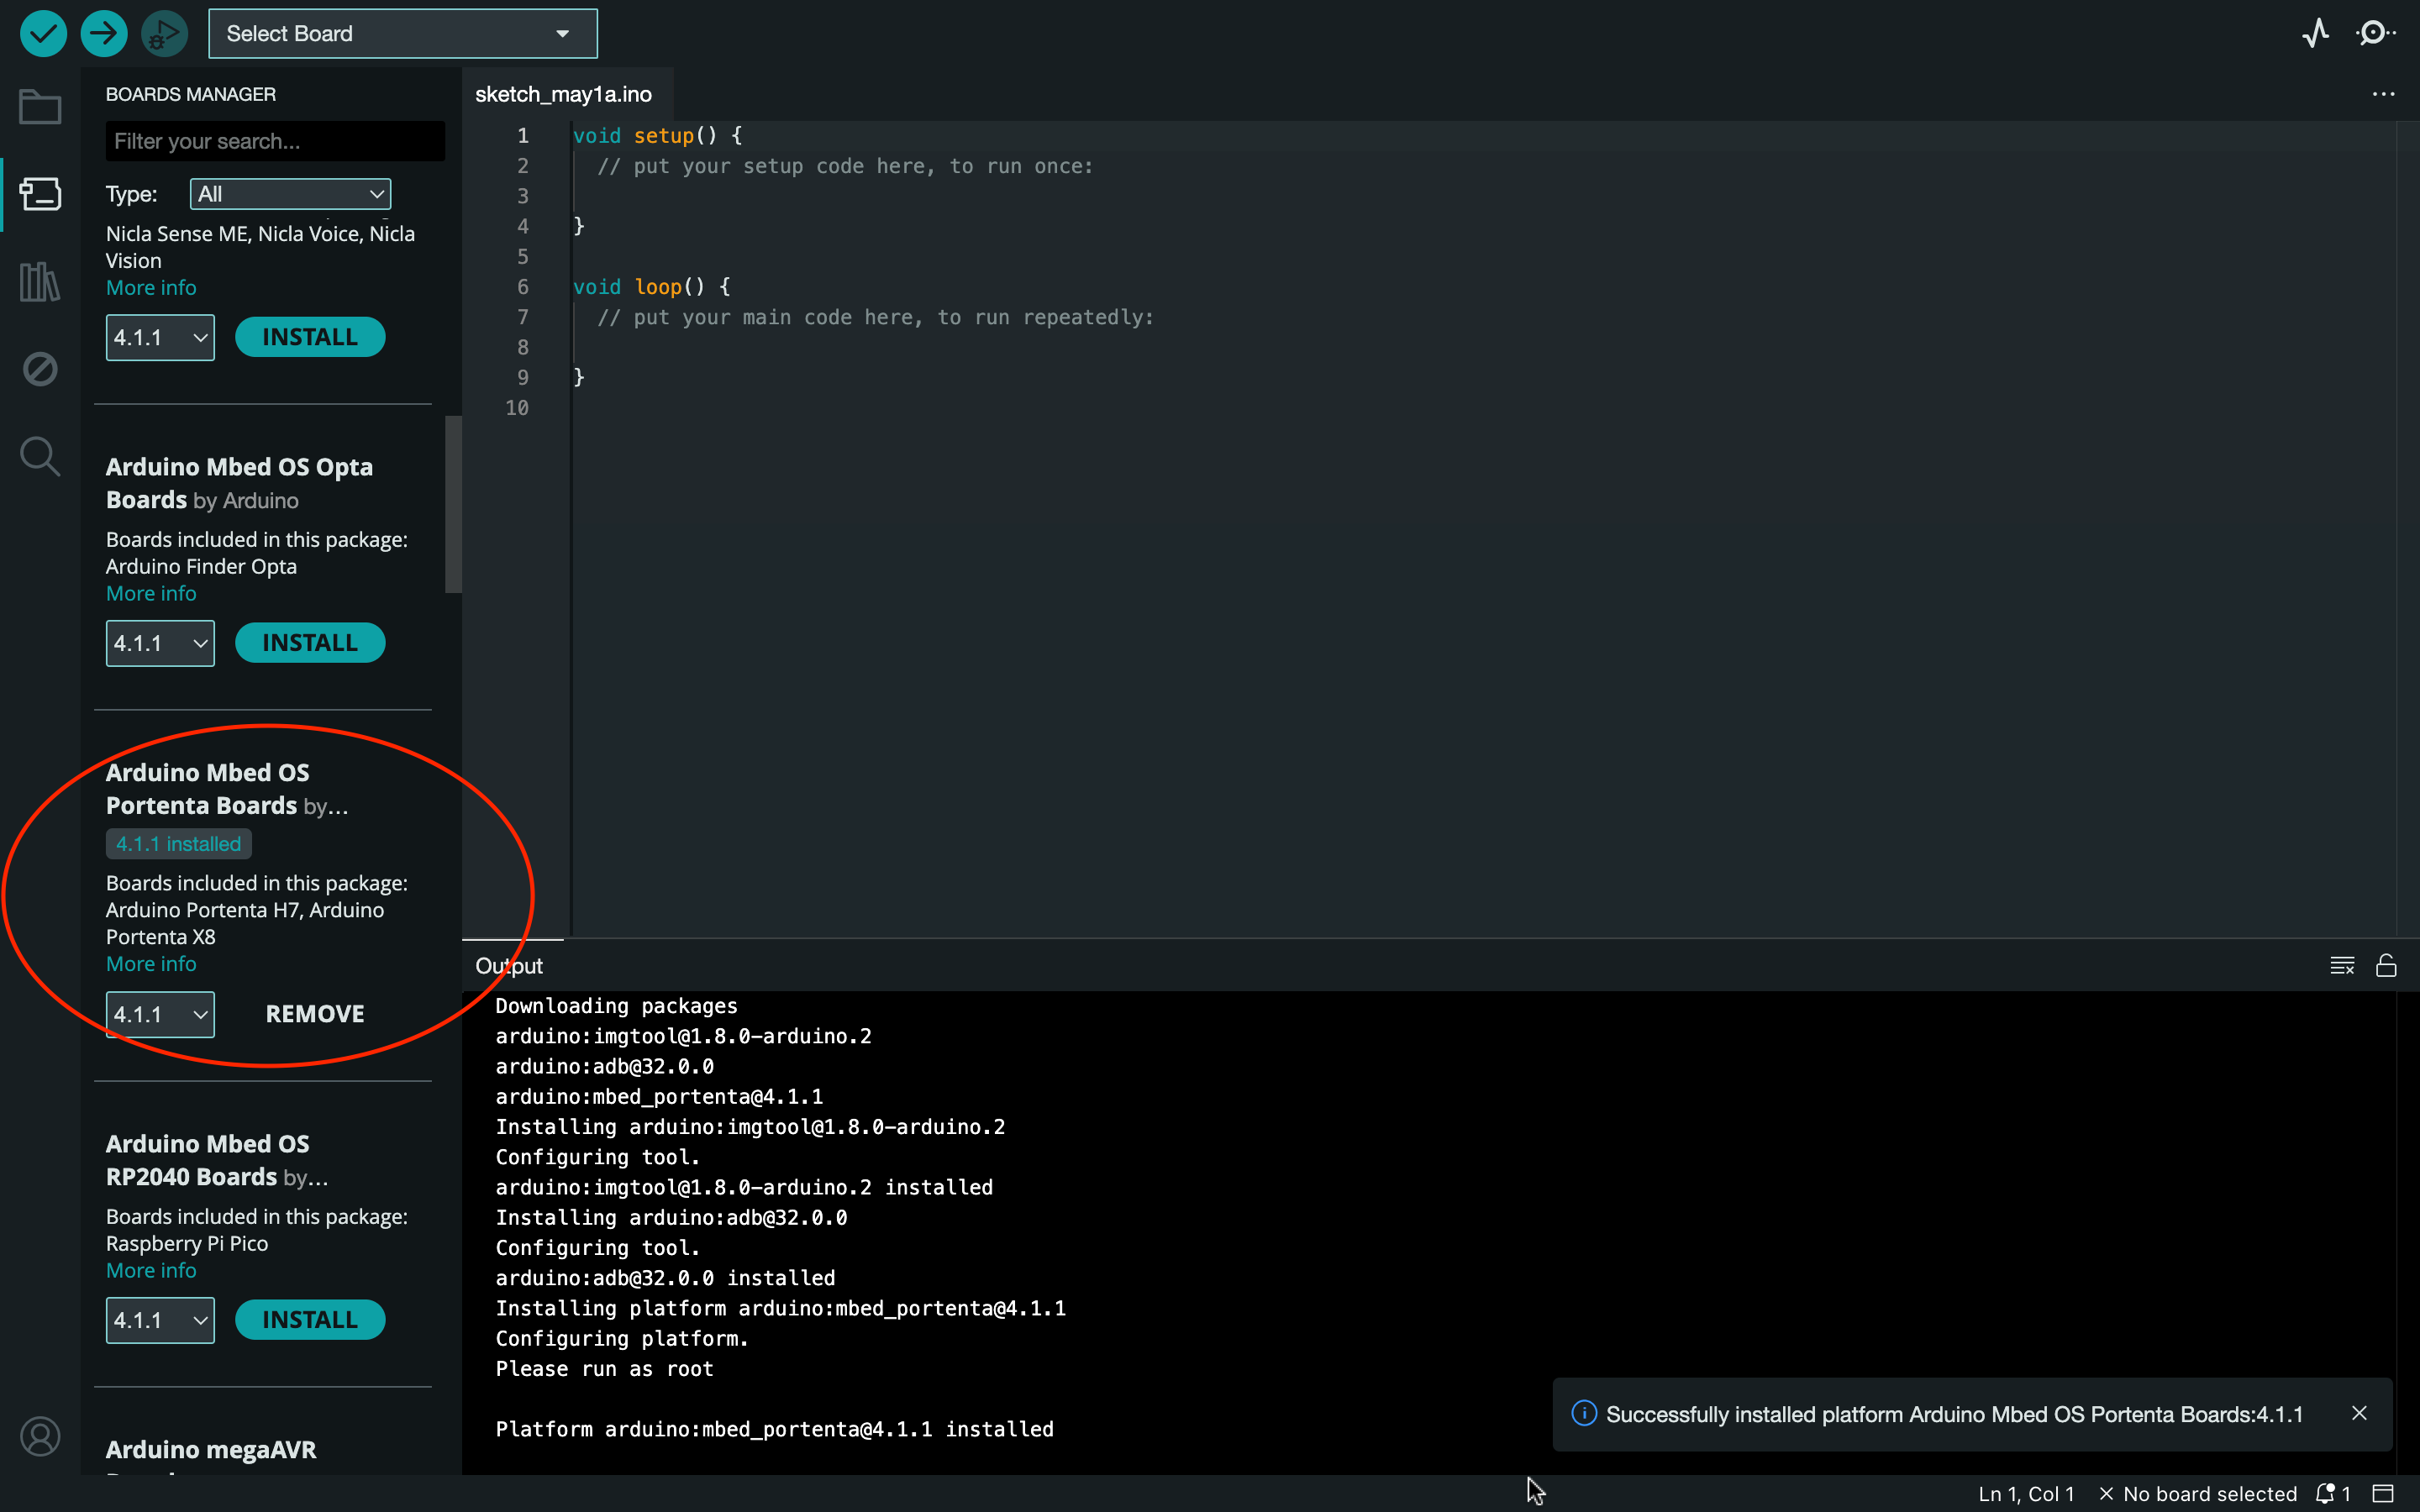
\includegraphics[width=0.7\linewidth]{images/ArduinoIDE/ArduinoMbedOSPortentaBoardsInstallation.png}
		\captionof{figure}{Installation Arduino Mbed OS Portenta Board}
		\label{Installation Arduino Mbed OS Portenta Board}
	\end{center}
\end{figure}



\subsection{Example Blink Sketch}

To upload the example sketch, go to File then click on examples and then click on 01.Basics and then select blink as shown in Figure ~\ref{Example LED-Test}. \\

\begin{figure}
	\begin{center}
		
		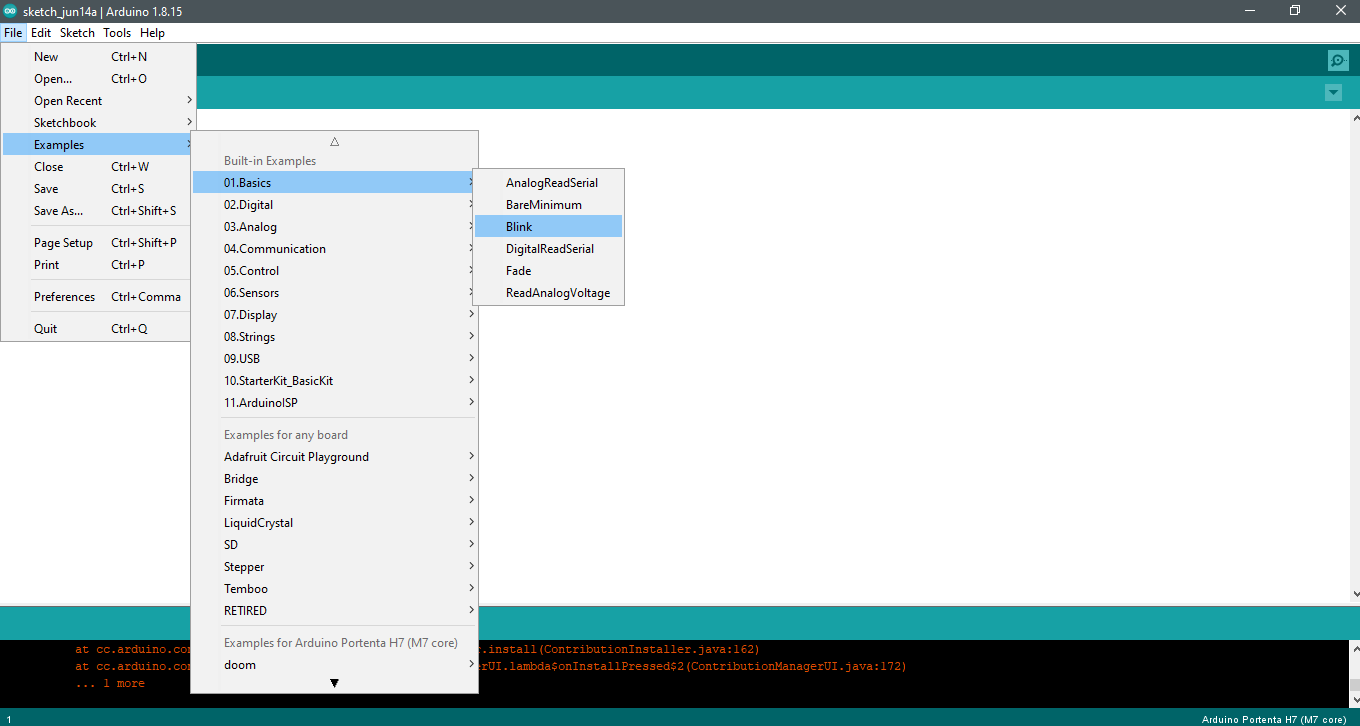
\includegraphics[width=0.7\linewidth]{images/ArduinoIDE/MenuBarOptions.png}
		\captionof{figure}{Example LED-Test}
		\label{Example LED-Test}
	\end{center}
\end{figure}


In the program, we initialize LED\_BUILTIN as the output in the setup function. In the loop function we turn on the LED by using digitalWrite() function. Click on upload and wait for it to complete. After the upload is done, the green LED on the board starts blinking with a delay of 1000ms.The blink sketch appears on the screen as shown in Figure \ref{Blink Sketch Compile}.
\begin{figure}
	\begin{center}
		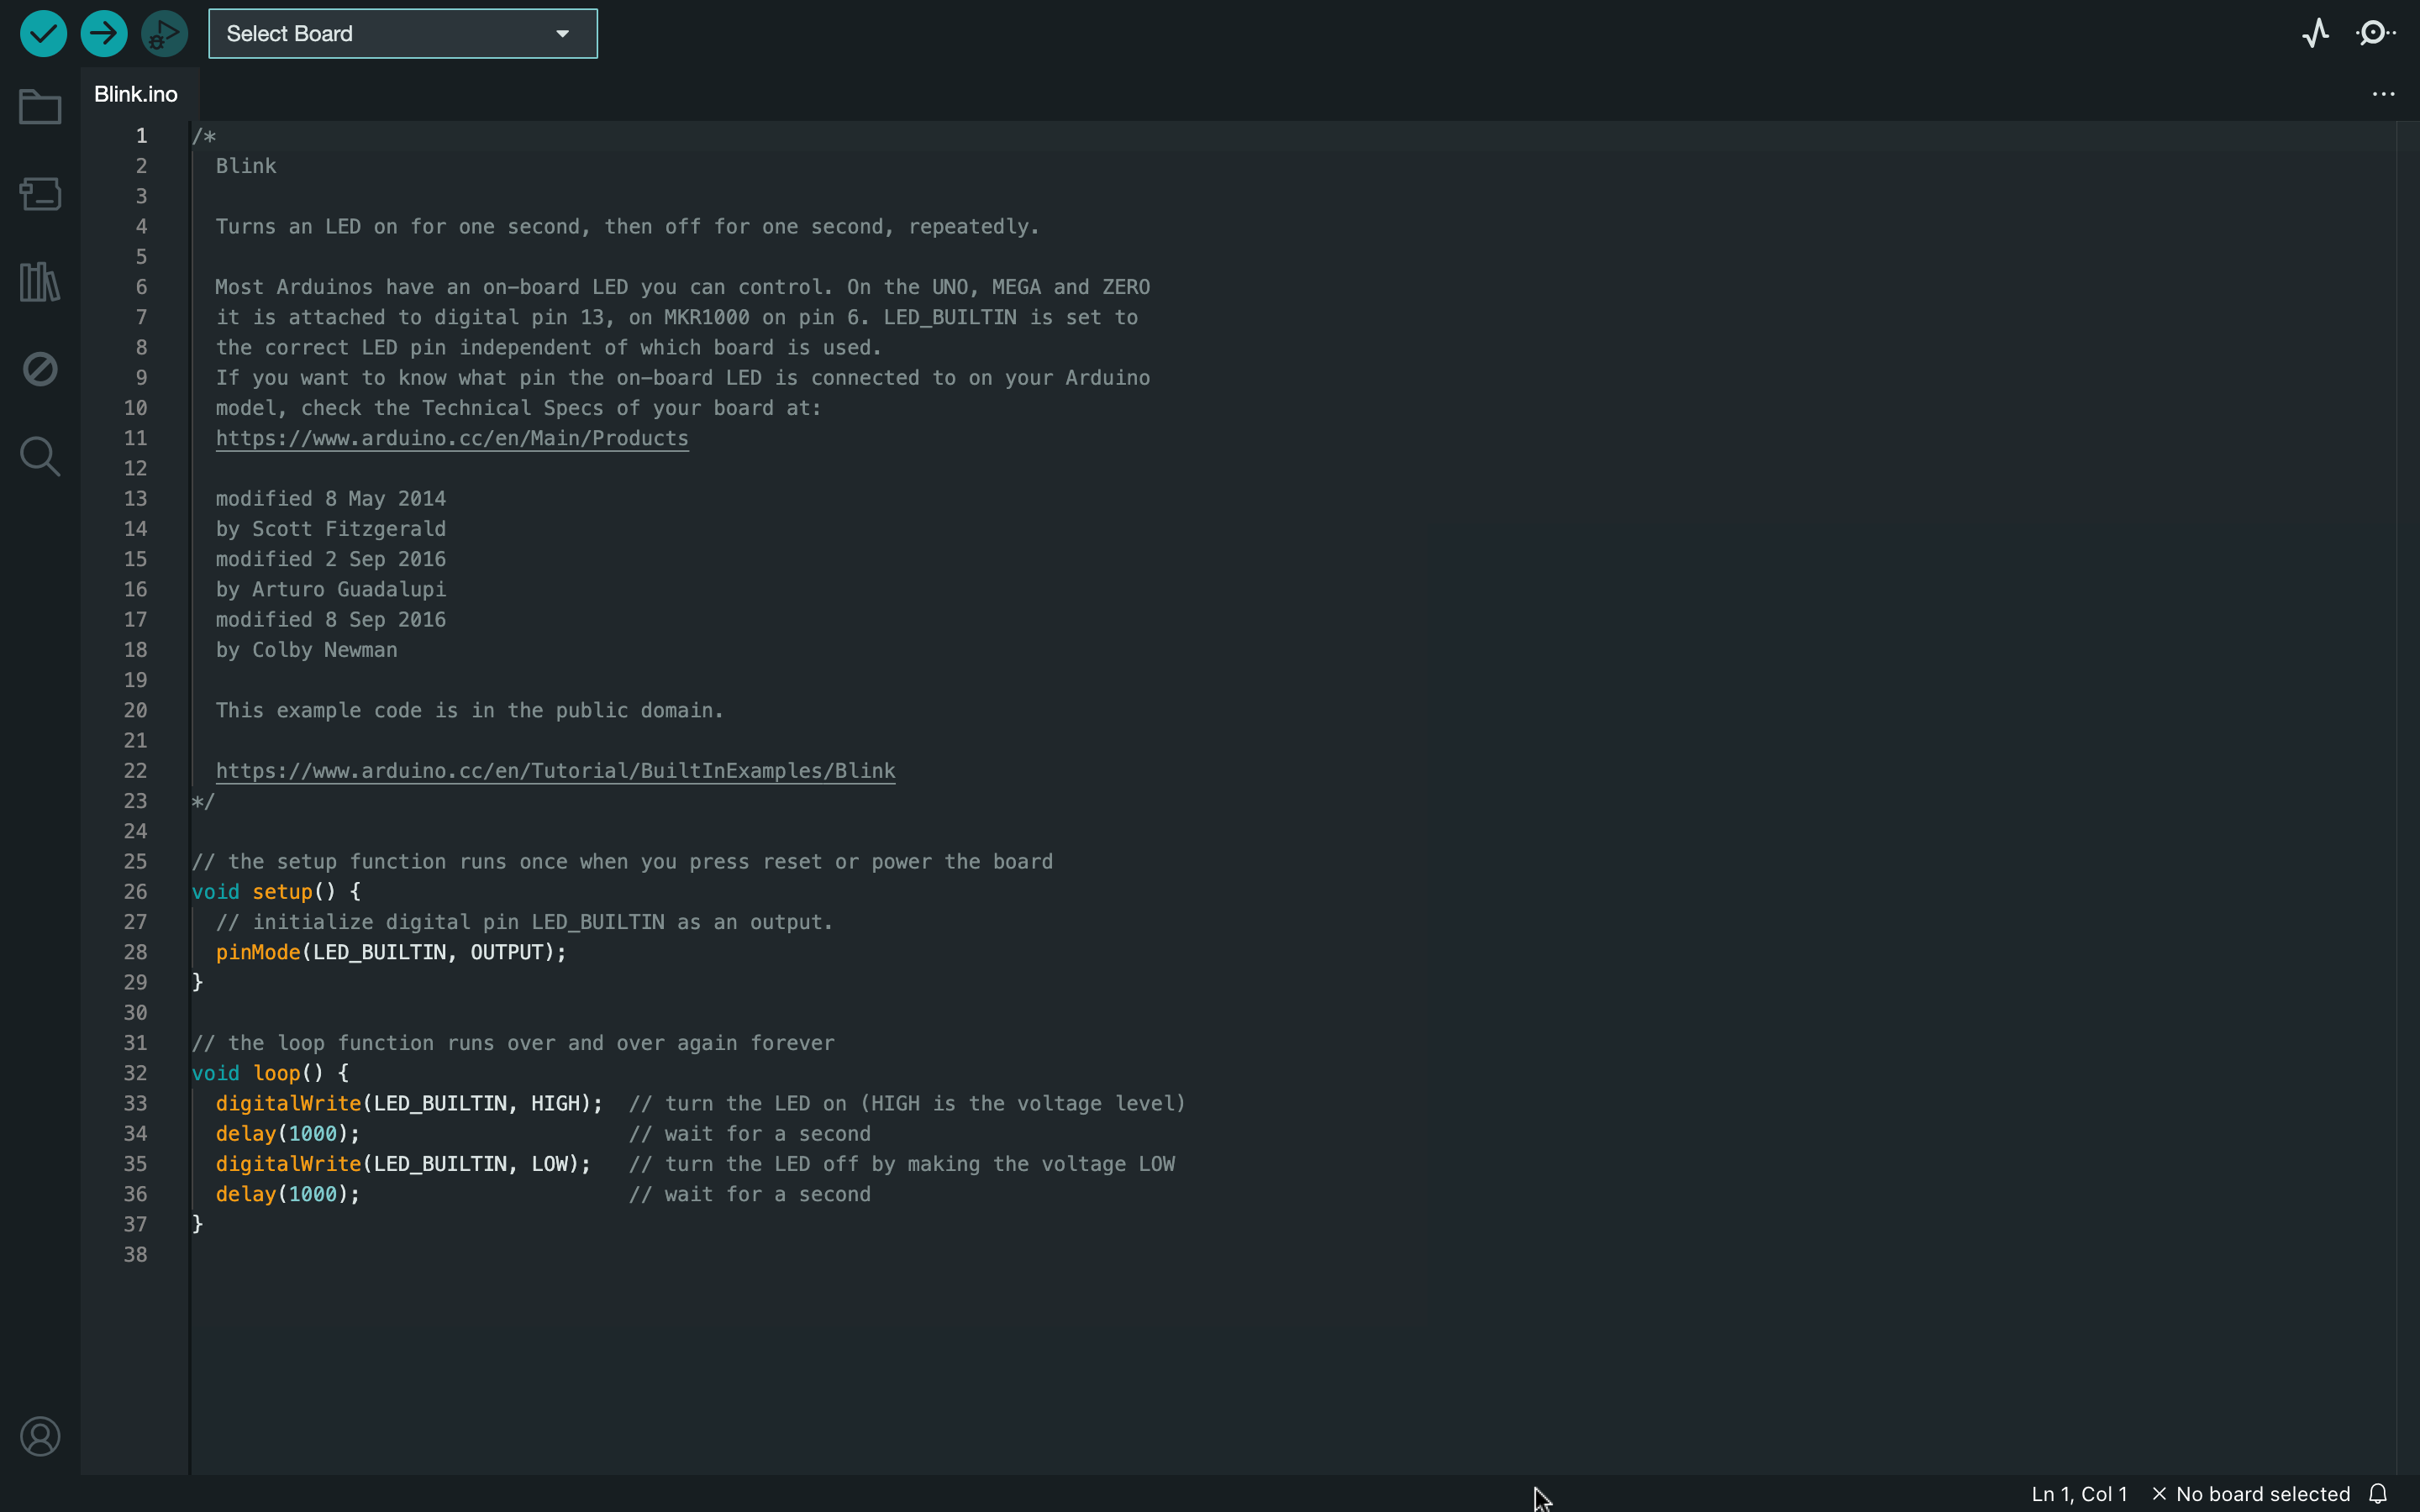
\includegraphics[width=0.7\linewidth]{images/ArduinoIDE/CompileBlinkSketch.png}
		\captionof{figure}{Blink Sketch Compile}
		\label{Blink Sketch Compile}
	\end{center}
\end{figure}



\section{Onboard Sensors with Examples}

\subsection{Murata 1DX Bluetooth® 5.1}
The onboard Bluetooth® module of the Portenta H7 offers low energy Bluetooth® functionality, in order to provide the board with the flexibility to be easily connected to devices which also support Bluetooth® Low Energy, such as the Arduino Nano 33 IoT or most modern smartphones. Compared to classic Bluetooth®, Low Energy Bluetooth® is intended to provide considerably reduced power consumption and cost while maintaining a similar communication range. \cite{bluetoothPortentaH7:2024}

\subsubsection{Overview}
In this Example we will enable low energy Bluetooth® on the Portenta H7 to allow an external Bluetooth® device to control the built-in LED either by turning it on or off.

\subsubsection{Goals}
\begin{itemize}
	\item Enabling Bluetooth® Low Energy connectivity on the Portenta H7.
	\item Connecting the Portenta to an external Bluetooth® Low Energy Mobile Application (In this case nRF Connect by Nordic Semiconductor).
\end{itemize}

\subsubsection{Required Hardware and Software}
\begin{itemize}
	\item Portenta H7 (ABX00042) or Portenta H7 Lite Connected (ABX00046)
	\item USB-C® cable (either USB-A to USB-C® or USB-C® to USB-C®)
	\item Arduino IDE 1.8.13+ or Arduino Pro IDE 0.0.4+
	\item Mobile device, phone or tablet
	\item nRFconnect or equivalent tool downloaded on your mobile device: nRF Connect for iOS or nRF Connect for android
\end{itemize}

\subsubsection{Instructions}
\begin{itemize}
	\item \textbf{Configuring the Development Environment:} To communicate with the Portenta H7 via Bluetooth®, you need to upload a pre-built sketch that starts a Bluetooth® network and allows your mobile device, which will be used to control the LEDs, to connect to it. The sketch uses the ArduinoBLE Library that enables the Bluetooth® Low Energy module and handles important functions, such as scanning, connecting and interacting with services provided by other devices. You will also be using a third party application (e.g. nRF Connect), running on your mobile device in order to connect your device to the board and help you control the built-in LED. ~\ref{Bluetooth-portentaH7}
	\begin{figure}
		\begin{center}
			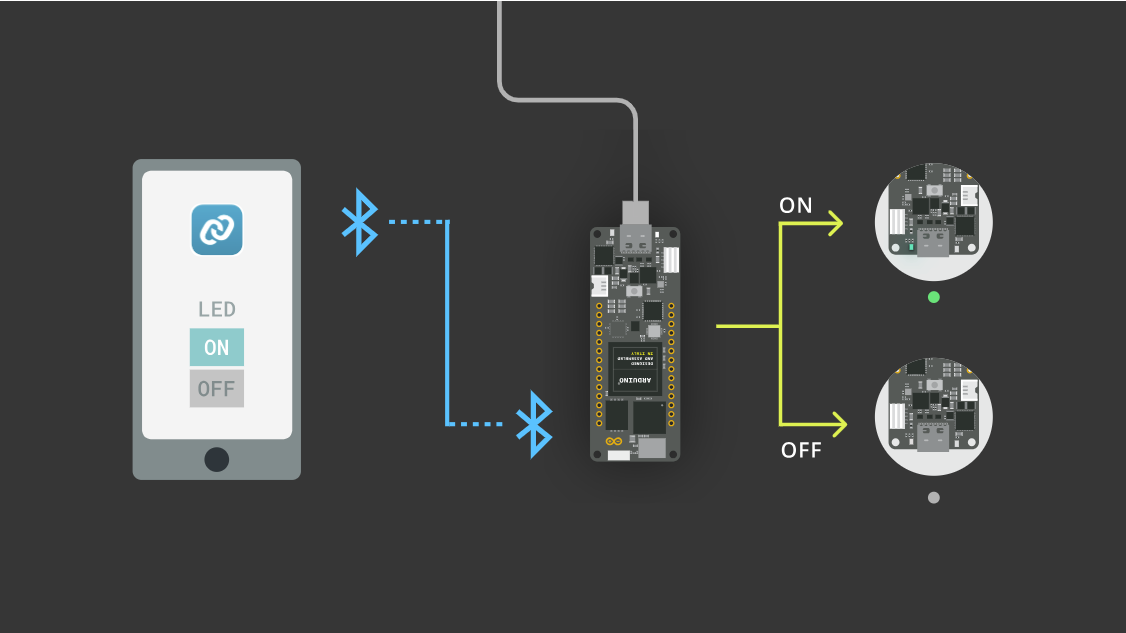
\includegraphics[width=0.7\linewidth]{Images/PortentaH7/Bluetooth-portentaH7.png}
			\caption{Bluetooth-portentaH7}
			\label{Bluetooth-portentaH7}\cite{bluetoothPortentaH7:2024}
		\end{center}
	\end{figure}
	
	\item \textbf{1. The Basic Setup:} Begin by plugging in your Portenta board to the computer using a USB-C® cable and open the Arduino IDE. If this is your first time running Arduino sketch files on the board, we suggest you check out how to set up the Portenta H7 for Arduino before you proceed.
	\begin{figure}
		\begin{center}
			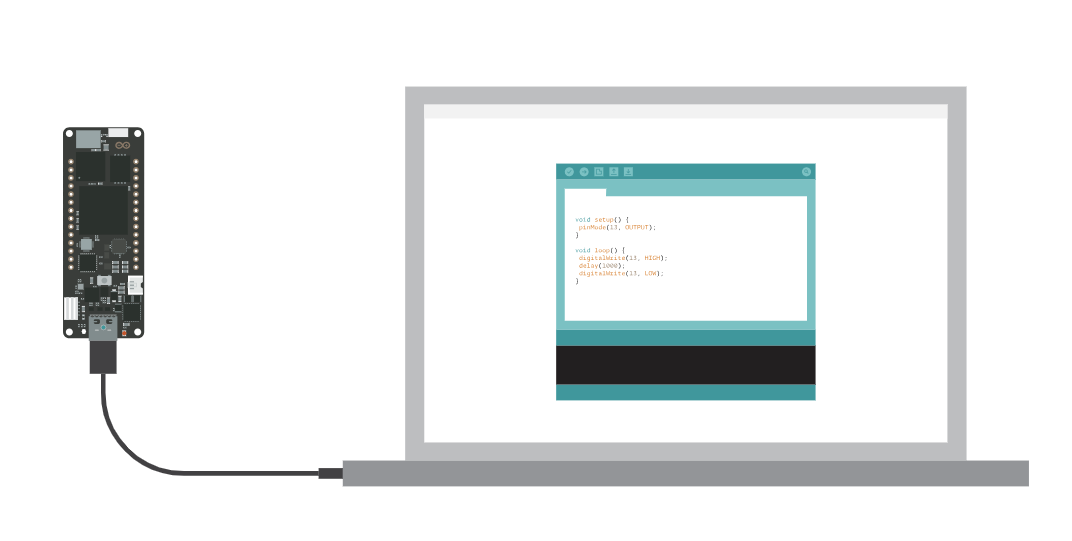
\includegraphics[width=0.7\linewidth]{Images/PortentaH7/PortentaH7-connection.png}
			\caption{PortentaH7-connection}
			\label{PortentaH7-connection}\cite{bluetoothPortentaH7:2024}
		\end{center}
	\end{figure}
	
	\item \textbf{2. Install the ArduinoBLE Library:} You will need to install the ArduinoBLE library in the Arduino IDE you are using. To install the library go to : \SHELL{ Tools > Manage Libraries...} type ArduinoBLE and click Install. Make sure you install ArduinoBLE version 1.1.3 or higher. ~\ref{Bluetooth-Library}
	\begin{figure}
		\begin{center}
			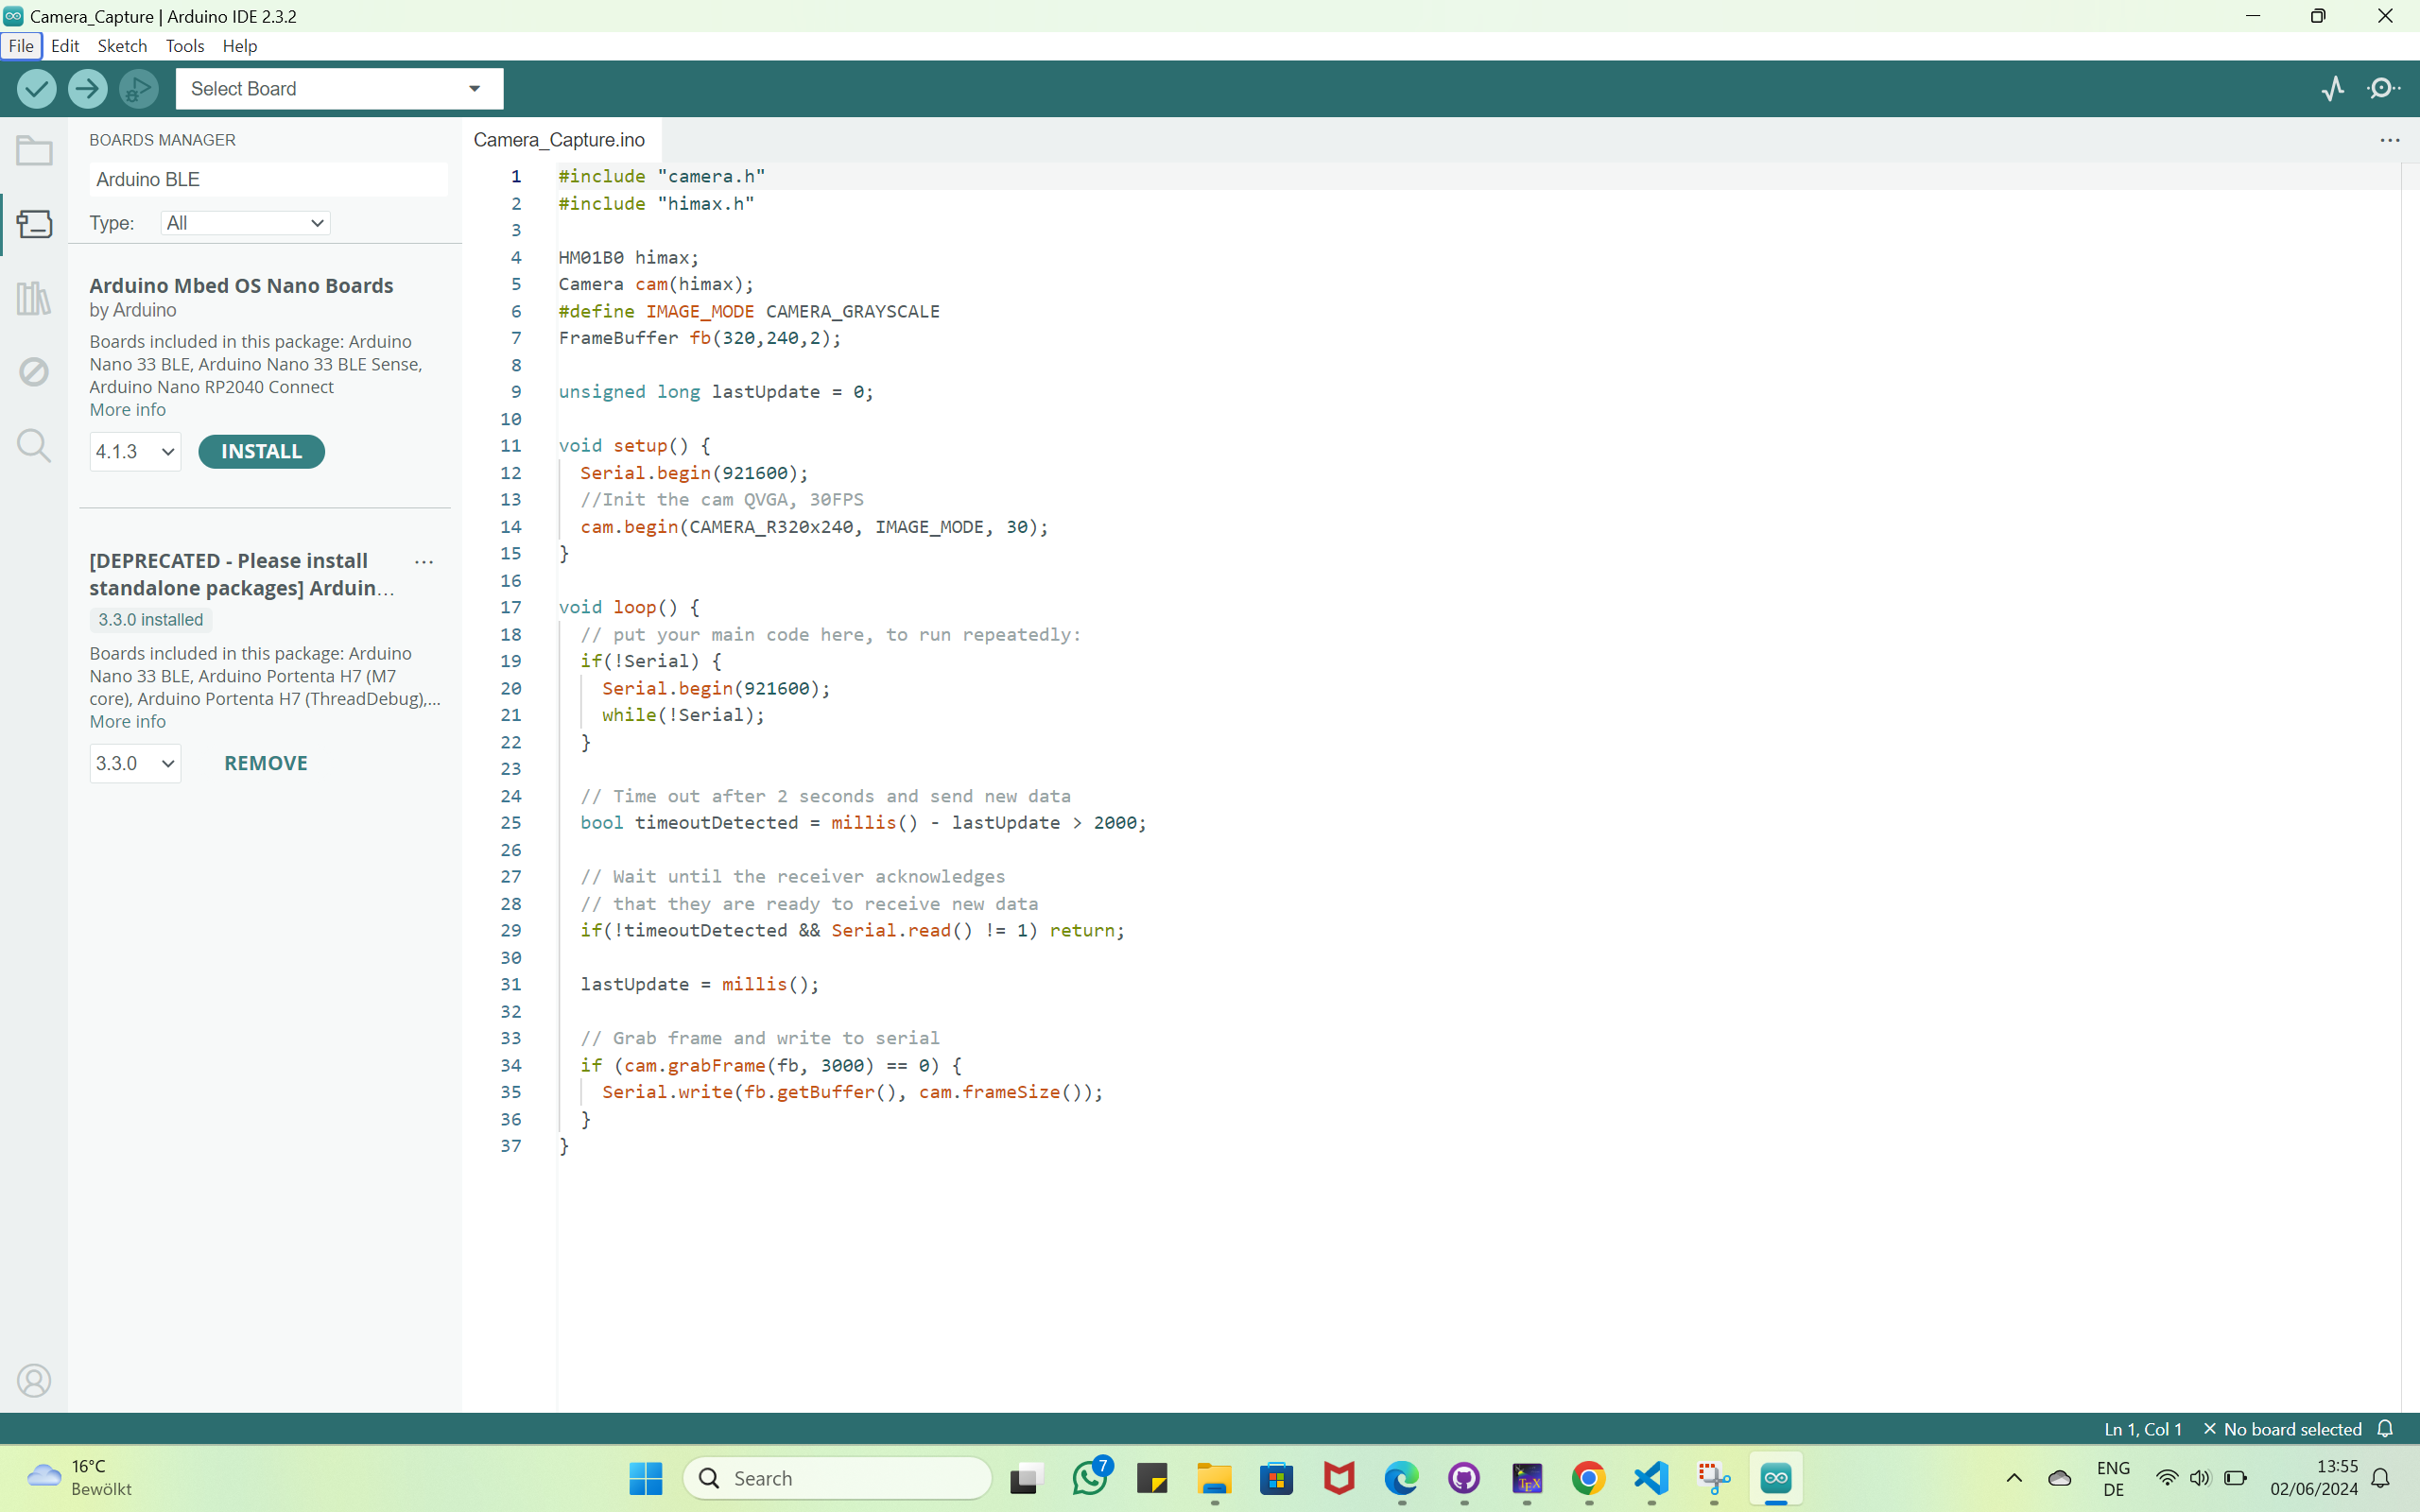
\includegraphics[width=0.7\linewidth]{Images/PortentaH7/Bluetooth-Library.png}
			\caption{Bluetooth-Library}
			\label{Bluetooth-Library}
		\end{center}
	\end{figure}
	
	\item \textbf{3. Create the Bluetooth® Low Energy Sketch:} Let's program the Portenta with the following example sketch. If the Bluetooth® Low Energy module has been initialized correctly, you will see the blue LED lighting up for one second after uploading the sketch. If it fails, you will see the red LED lighting up instead. Copy and paste the following code into a new sketch in your IDE or download it from Arduino-Pro-Tutorials in the Arduino IDE and open it from: \SHELL{Examples > Arduino-Pro-Tutorials > BLE Connectivity on Portenta H7 > PortentaBLE }
	\begin{lstlisting}
		#include <ArduinoBLE.h>
		
		BLEService ledService("19b10000-e8f2-537e-4f6c-d104768a1214");
		
		// Bluetooth Low Energy LED Switch Characteristic - custom 128-bit UUID, read and writable by central
		BLEByteCharacteristic switchCharacteristic("19b10000-e8f2-537e-4f6c-d104768a1214", BLERead | BLEWrite);
		
		const int ledPin = LED-BUILTIN; // Pin to use for the LED
		
		void setup() {
			Serial.begin(9600);
			//while (!Serial);   // Uncomment to wait for serial port to connect.
			
			// Set LED pin to output mode
			pinMode(ledPin, OUTPUT);
			digitalWrite(ledPin, HIGH);
			
			// Begin initialization
			if (!BLE.begin()) {
				Serial.println("Starting Bluetooth Low Energy failed!");
				digitalWrite(LEDR, LOW);
				delay(1000);
				digitalWrite(LEDR, HIGH);
				
				// Stop if Bluetooth Low Energy couldn't be initialized.
				while (1);
			}
			
			// Set advertised local name and service UUID:
			BLE.setLocalName("LED-Portenta-01");
			BLE.setAdvertisedService(ledService);
			
			// Add the characteristic to the service
			ledService.addCharacteristic(switchCharacteristic);
			
			// Add service
			BLE.addService(ledService);
			
			// Set the initial value for the characeristic:
			switchCharacteristic.writeValue(0);
			
			// start advertising
			BLE.advertise();
			digitalWrite(LEDB, LOW);
			delay(1000);
			digitalWrite(LEDB, HIGH);
			Serial.println("BLE LED Control ready");
		}
		
		void loop() {
			// Listen for Bluetooth Low Energy peripherals to connect:
			BLEDevice central = BLE.central();
			
			// If a central is connected to peripheral:
			if (central) {
				Serial.print("Connected to central: ");
				// Print the central's MAC address:
				Serial.println(central.address());
				digitalWrite(LEDB, HIGH);
				delay(100);
				digitalWrite(LEDB, LOW);
				delay(100);
				digitalWrite(LEDB, HIGH);
				
				// While the central is still connected to peripheral:
				while (central.connected()) {
					// If the remote device wrote to the characteristic,
					// Use the value to control the LED:
					if (switchCharacteristic.written()) {
						if (switchCharacteristic.value()) {   // Any value other than 0
							Serial.println("LED on");
							digitalWrite(ledPin, LOW);          // Will turn the Portenta LED on
						} else {                             
							Serial.println("LED off");
							digitalWrite(ledPin, HIGH);         // Will turn the Portenta LED off          
						}
					}
				}
				
				// When the central disconnects, print it out:
				Serial.print("Disconnected from central: ");
				Serial.println(central.address());    
				digitalWrite(LEDB, HIGH);
				delay(100);
				digitalWrite(LEDB, LOW);
				delay(100);
				digitalWrite(LEDB, HIGH);
			}
		}    
		
	\end{lstlisting}
	
	In this example, you use a pre-defined Bluetooth number code pre-setup for controlling a device's LED. This code can also be referred to as GATT codes, which define how two Bluetooth® low energy devices transfer data. Once a connection is established with a device, its respective GATT code, which is a 16 bit identifier, is stored in a lookup table for future reference.
	
	These GATT codes are very long, but, in this example, it is always the same code:
	\begin{lstlisting}
		BLEService ledService("19b10000-e8f2-537e-4f6c-d104768a1214"); // BLE LED Service
	\end{lstlisting}	
	
	\item \textbf{4. Upload the Sketch:} Double press the reset button so the built-in LED is slowly pulsing green. Then, select your board in the menu: \SHELL{Tools > Board > Arduino Portenta H7 (M7 core)} ~\ref{select-board-h7}
	\begin{figure}
		\begin{center}
			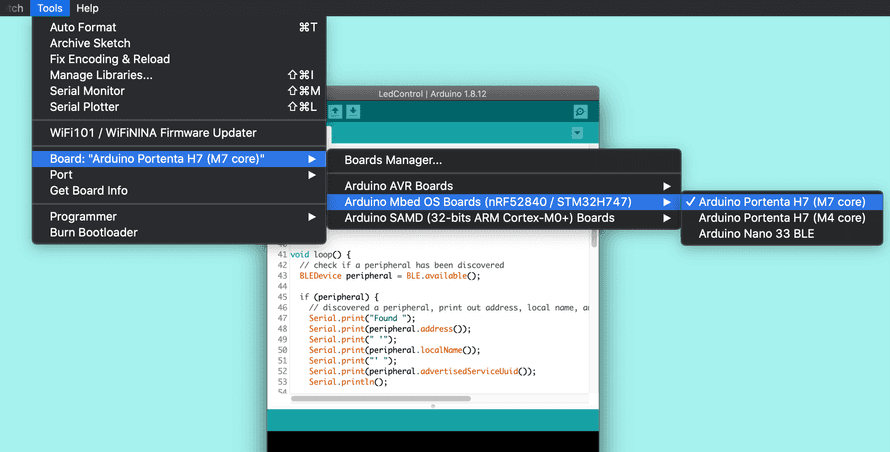
\includegraphics[width=0.7\linewidth]{Images/PortentaH7/select-board-h7.png}
			\caption{select-board-h7}
			\label{select-board-h7}
		\end{center}
	\end{figure}
	
	Choose the Port where your Portenta is connected to and Upload the sketch. Open the Serial Monitor once you have uploaded the code to the board to see debugging messages. If the Bluetooth® Low Energy setup was successful, you should see the message BLE LED Control ready. If something went wrong, you will see the message Starting Bluetooth Low Energy failed!. In that case update the Arduino BLE library (in the Library Manager) and the board (in the Board Manager) to the latest version and try again. ~\ref{select-port}
	
	\begin{figure}
		\begin{center}
			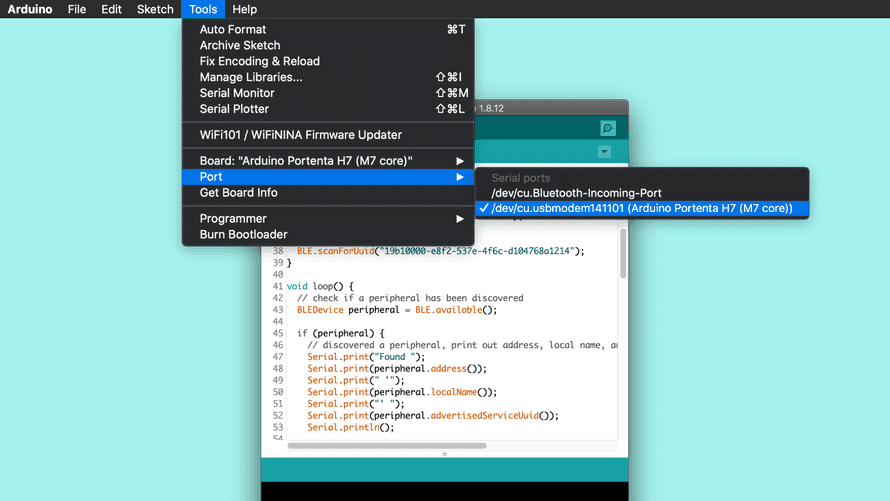
\includegraphics[width=0.7\linewidth]{Images/PortentaH7/select-port.png}
			\caption{select-port}
			\label{select-port}
		\end{center}
	\end{figure}
	
	\item \textbf{5.  Connect an External Device :} On your mobile device install nRF Connect or an equivalent app that allows for Bluetooth Low Energy connections. We will refer to nRF Connect for the rest of this tutorial. ~\ref{NRF-Connect}
	\begin{figure}
		\begin{center}
			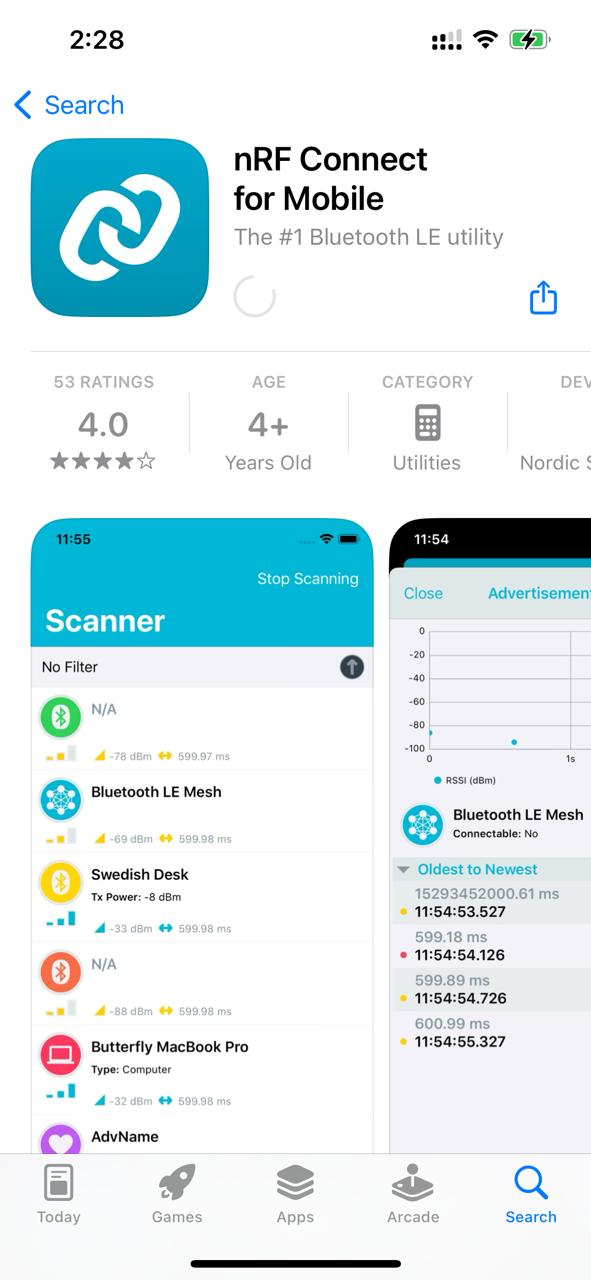
\includegraphics[width=0.7\linewidth]{Images/PortentaH7/NRF-Connect.jpg}
			\caption{NRF-Connect}
			\label{NRF-Connect}
		\end{center}
	\end{figure}
	Once you have downloaded the nRF application on your mobile device, look for your Portenta in the device list. You may filter the list by "Portenta" to easierly find your board in case you are using nRF Connect.
	
	\item When you find your board in the list tap "Connect".
	\item Navigate to the "Services" screen and tap the arrow up button.
	\item Switch to "Bool" type and move the toggle to "True". Confirm the dialog with a tap on "Write" and you should see the built-in LED turned on. If you do the same procedure again but setting the toggle switch to "False", it will turn off the LED. ~\ref{Bluetooth-scan}
	\begin{figure}
		\begin{center}
			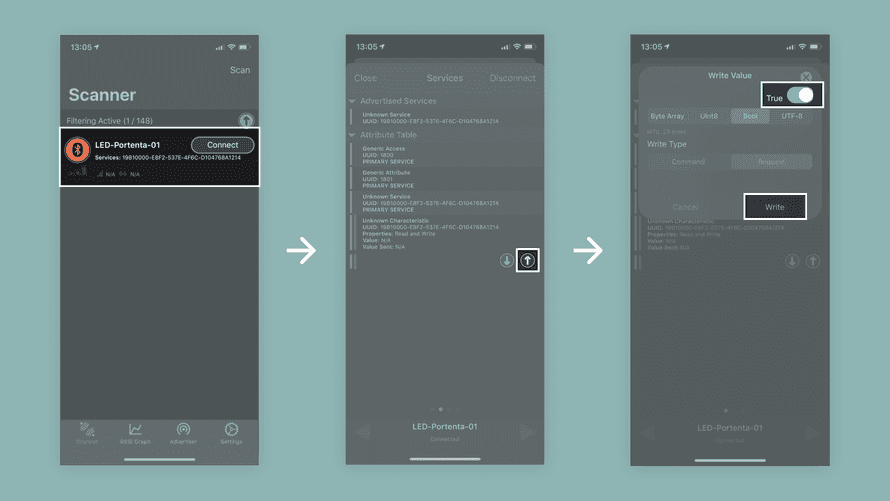
\includegraphics[width=0.7\linewidth]{Images/PortentaH7/Bluetooth-scan.png}
			\caption{Bluetooth-scan}
			\label{Bluetooth-scan}
		\end{center}
	\end{figure}
	\item \textbf{6. Conclusion:} This example shows how to connect and control the built-in LED using a Bluetooth Low Energy connection. You have learned how a simple Bluetooth Low Energy connection between your Portenta and your cell phone, which has basic communication abilities between the two devices, works. ~\ref{NRF-Connect}	
	
\end{itemize}

\end{comment}



%\section{First Step with PortentaH7:}
%
%\subsection{Setting Up Portenta H7 For Arduino:}
%This Example teaches you how to set up the board, how to configure your computer and how to run the classic Arduino blink example to verify if the configuration was successful. ~\ref{PortentaH7-connection} \cite{portentaSetup:2024}
%\subsection{Goals:}
%\begin{itemize}
%	\item About the Arduino and Mbed operating system (Mbed OS) stack
%	\item Installing the Mbed library
%	\item Controlling the built in LED on the Portenta board
%\end{itemize}
%\subsection{Instructions:}
%\begin{itemize}
%	\item \textbf{Configuring the Development Environment:} In this section, we will guide you through a step-by-step process of setting up your Portenta board for running an Arduino Sketch that blinks the built-in RGB LED.
%	\item \textbf{The Basic Setup:} Let's begin by Plug-in your Portenta to your computer using the appropriate USB-C® cable. Next, open your IDE and make sure that you have the right version of the Arduino IDE downloaded on to your computer.
%	\begin{figure}
%		\begin{center}
%			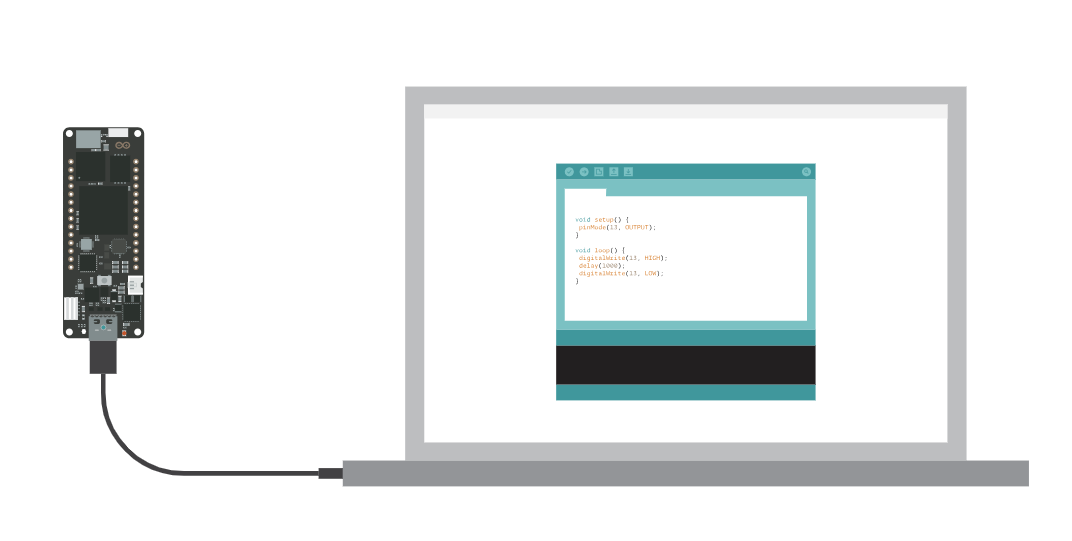
\includegraphics[width=0.7\linewidth]{Images/PortentaH7/PortentaH7-connection.png}
%			\caption{PortentaH7-connection}
%			\label{PortentaH7-connection}
%		\end{center}
%	\end{figure}
%	\item \textbf{Adding the Portenta to the List of Available Boards:} In your Arduino IDE, open the board manager and search for "portenta". Find the Arduino mbed-enabled Boards library and click on "Install" to install the latest version of the mbed core (1.2.3 at the time of writing this tutorial). ~\ref{Portentaport}
%	\begin{figure}
%		\begin{center}
%			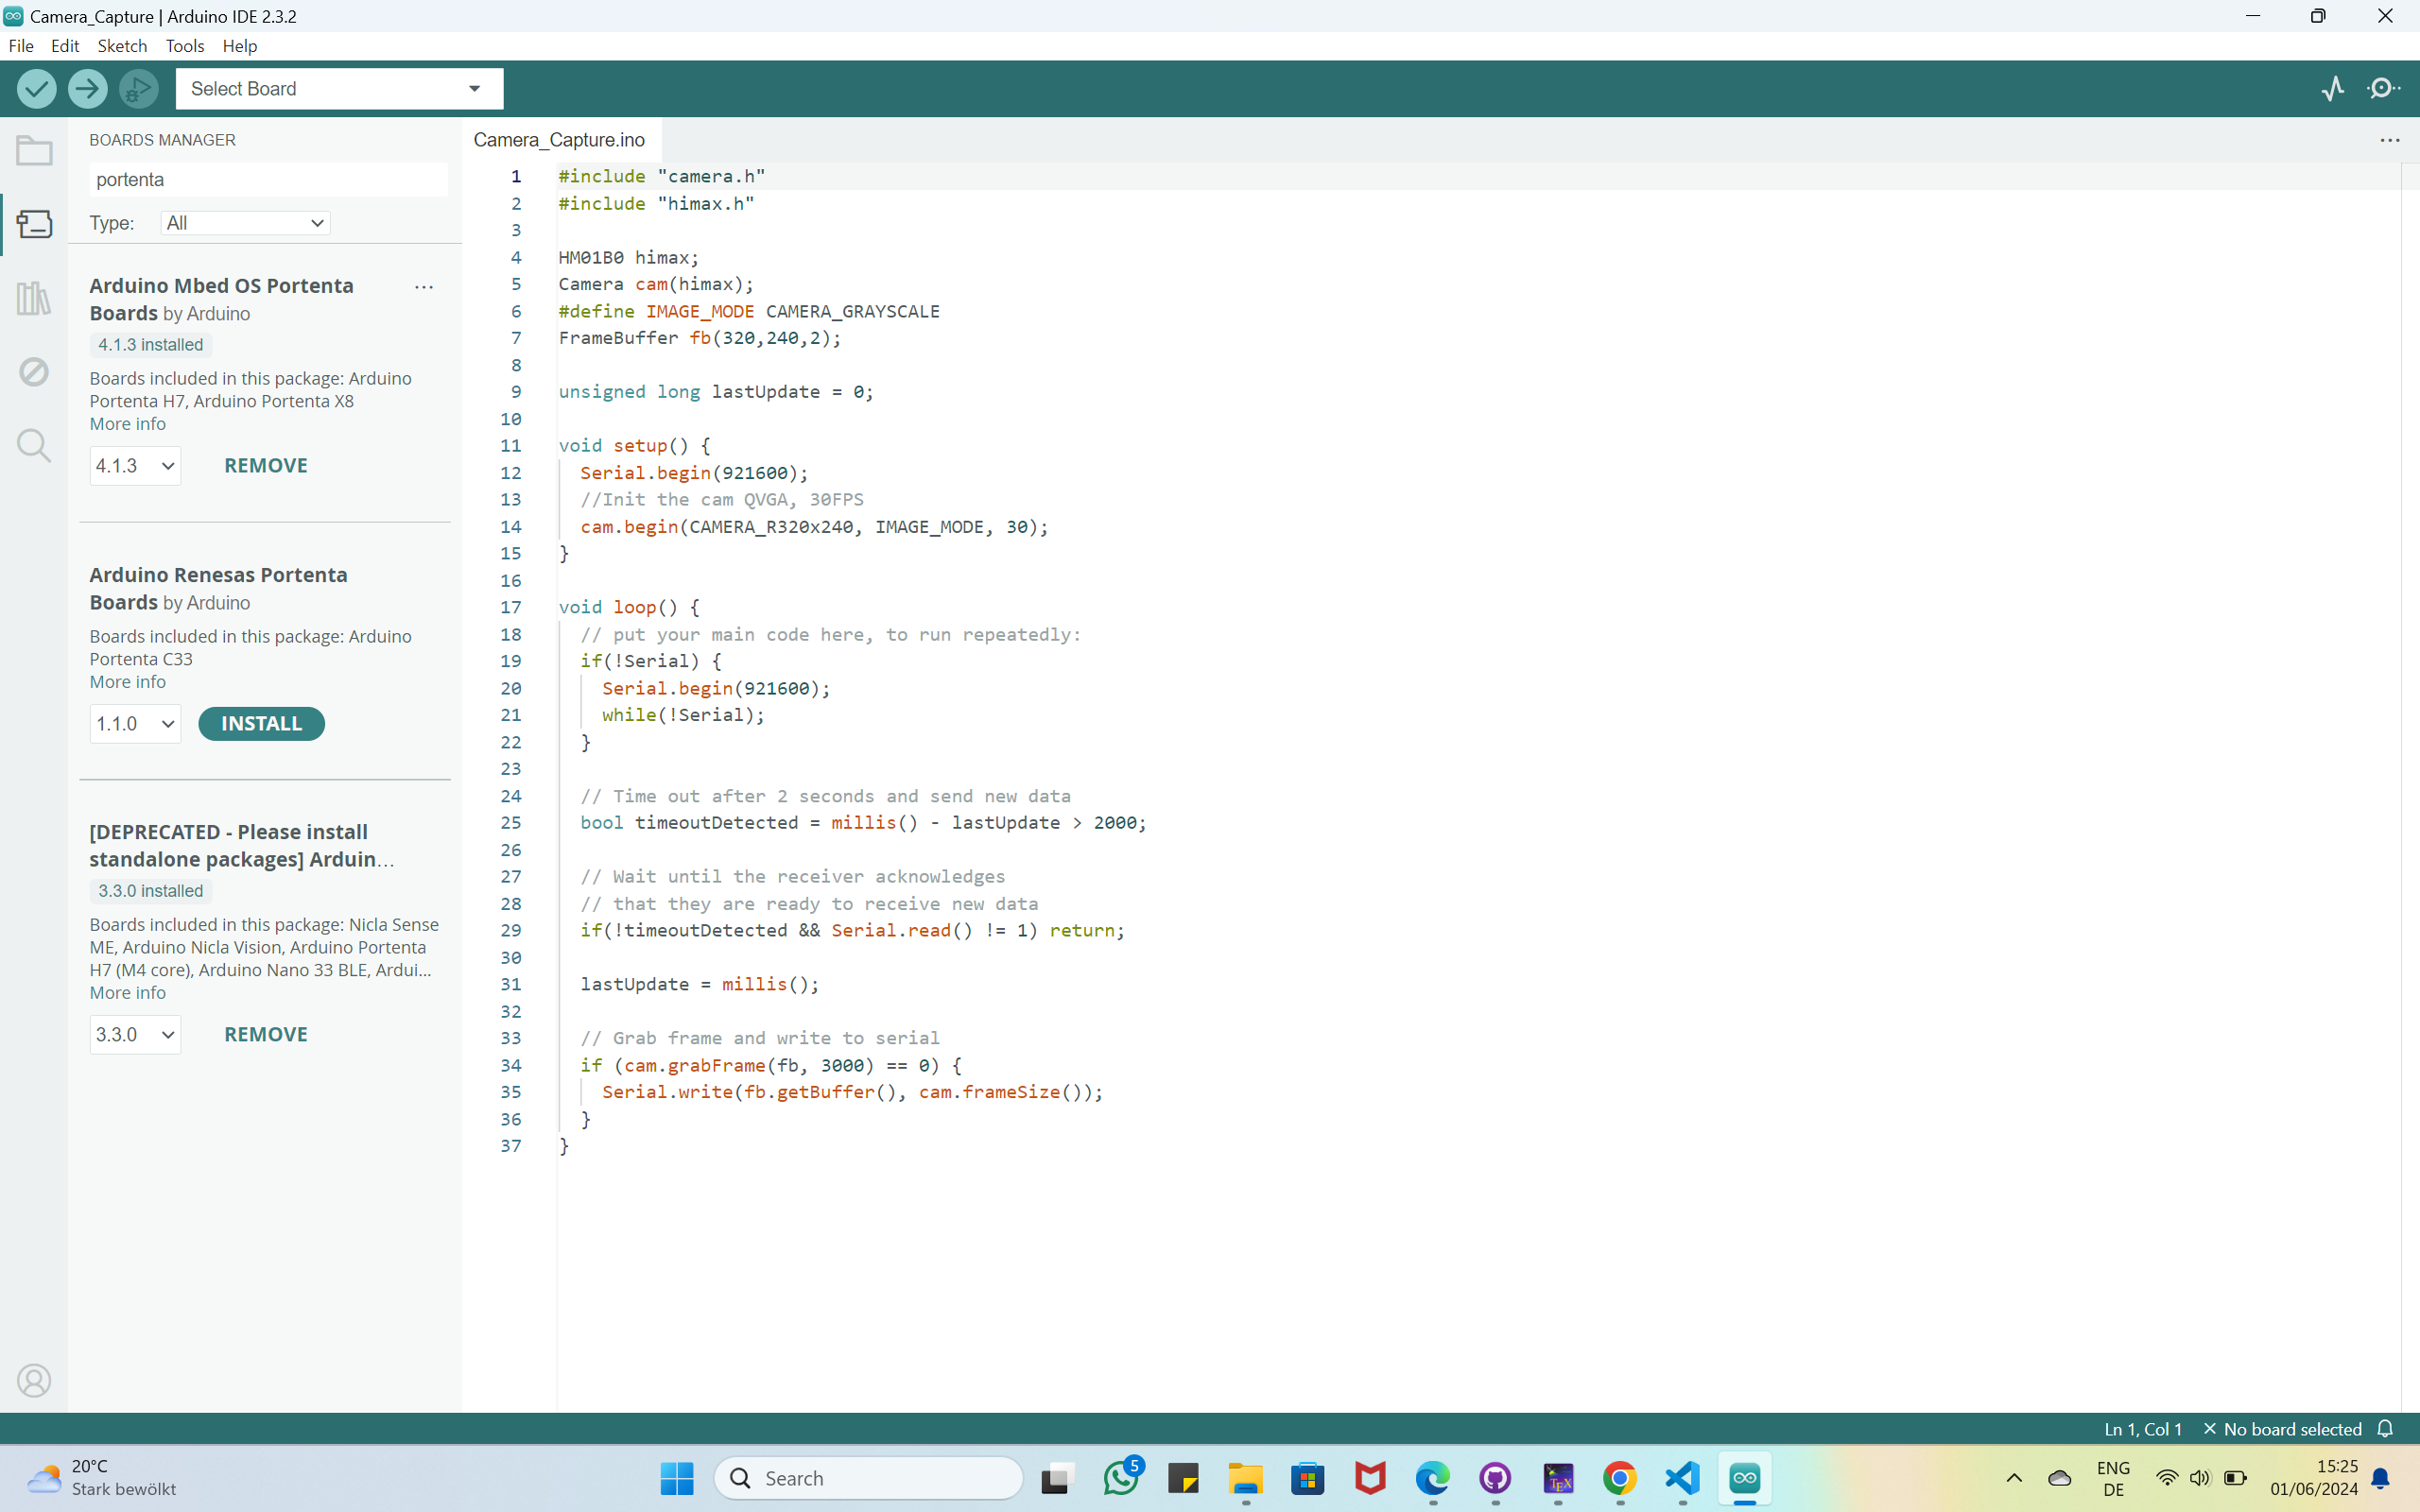
\includegraphics[width=0.7\linewidth]{Images/PortentaH7/Portentaport.png}
%			\caption{Portentaport}
%			\label{Portentaport}
%		\end{center}
%	\end{figure}
%	
%	\item \textbf{Uploading the Classic Blink Sketch:} Let's program the Portenta with the classic blink example to check if the connection to the board works. 
%	
%	\begin{lstlisting}
%		// the setup function runs once when you press reset or power the board
%		void setup() {
%			// initialize digital pin LED_BUILTIN as an output.
%			pinMode(LED_BUILTIN, OUTPUT);
%			digitalWrite(LED_BUILTIN, HIGH); // turn the LED off after being turned on by pinMode()
%		}
%		
%		// the loop function runs over and over again forever
%		void loop() {
%			digitalWrite(LED_BUILTIN, LOW); // turn the LED on (LOW is the voltage level)
%			delay(1000); // wait for a second
%			digitalWrite(LED_BUILTIN, HIGH); // turn the LED off by making the voltage HIGH
%			delay(1000); // wait for a second
%		}   
%		
%	\end{lstlisting}
%	
%\end{itemize}

%\subsection{Conclusion:}
%You have now configured your Portenta board to run Arduino sketches. Along with that you gained an understanding of how the Arduino Core runs on top of Mbed OS.